\section{Alignment Training for Controllable Generation}
\label{sec:nlgcg}

In the previous section, we showed how to make an arbitrary
\sequencetosequence~model more likely to generate semantically correct
utterances using data-augmentation. While the resultant generation model is
more faithful, it still lacks even coarse-grained control over the organization
of the generated utterance.  What's more, there's no guarantee that small
changes to the input don't lead to dramatically different outputs.  For
example, changing a boolean attribute, e.g. changing
\AV{\textit{family\_friendly}}{\textit{yes}} to
\AV{\textit{family\_friendly}}{\textit{no}}, may lead to dramatically different
syntactic structure in the output.  This is because the structure or plan of
the utterance is only determined implicitly by the
\sequencetosequence~decoder's language model.

In this section, we show how to make a \sequencetosequence~controllable, which
we achieve through a particular linearization of the input
\meaningrepresentation, a linearization strategy we call \textit{alignment
training}. That is, we can specify the order in which the \attributevalues~of
an input \meaningrepresentation~are to be realized in the utterance.  See
\autoref{fig:examplecontrol} for example realizations from a controllable
generation model that follow three different permutations of \Atr{name},
\Atr{eat\_type}, and \Atr{area} attributes.  Through evaluation on two dialogue
generation benchmarks we show that alignment training yields high levels of
control in both GRU and Transformer models. This holds when models follow
either a separate planning model or a human provided plan.

We also propose using a phrase-based data augmentation method to further
improve the robustness of control. We further evaluate the control mechanism on
randomly generated plans which are much harder to follow than human or model
provided plans. We find that phrase-based data augmentation helps
\sequencetosequence~models follow these more difficult plans.

\subsection{Alignment Training Linearization}

Unlike the arbitrary linearization used in \autoref{sec:fgtgm},
\alignmenttraining~linearization~is not solely a function of $\mr$, but is
determined by both $\mr$ and a reference utterance $\utttoks$. Given a
$\left(\mr, \utttoks\right)$ pair, the \alignmenttraining~linearization finds a
linearization $\ls$ such that the order of the \attributevalues~in $\ls(\mr)$
corresponds to the order in which they are realized in $\utttoks$. 

\begin{figure}[p]
    \fbox{\begin{minipage}{\textwidth}
\center

\begin{minipage}{0.98\textwidth}
\begin{subfigure}{\textwidth}
\caption{Example of an alignment training linearization for a \meaningrepresentation~with a list-valued attribute, \textit{genres}. Note also that the \textit{rating} attribute for ViGGO examples is not aligned but always appended after the dialogue act (see \autoref{sec:align} for details). }
\center
\begin{minipage}[t]{0.48\textwidth}
\small
$\mr = \left[\!\!\left[\begin{array}{l} 
    \textsc{Give Opinion} \\ 
    \textrm{name=Little Nightmares} \\
    \textrm{rating=good} \\
    \textrm{genres=[}\\
    \textrm{~~~~adventure,} \\
    \textrm{~~~~platformer,}\\
    \textrm{~~~~puzzle} \\
    \textrm{]} \\
    \textrm{player\_perspective=side view}
\end{array}\right]\!\!\right]$ 
\end{minipage}
\hfill
\begin{minipage}[t]{0.48\textwidth}
\small
$\ls(\mr) = \left[ \begin{array}{l}
\starttok, \\
\textit{give\_opinion},\\
\textit{rating=good},\\ 
\textit{name=Little Nightmares},  \\
\textit{genres=adventure},  \\
\textit{player\_perspective=side view},\\
\textit{genres=platformer},  \\
\textit{genres=puzzle},  \\
\stoptok\end{array} \right]
$ 
\end{minipage}\\
\begin{minipage}[t]{\textwidth}
~\\[0pt]
$\utttoks = $ \textit{Little Nightmares is a pretty cool game that has kept me entertained. It's an adventure side-scrolling platformer with some puzzle elements to give me a bit of a challenge.}
\end{minipage}
\end{subfigure}

~\\~\\


\begin{subfigure}{\textwidth}
\caption{Example of an alignment training linearization with repeated attribute-values. In this case, the \textit{name} attribute is realized twice and 
so it appears twice in the linearization.}
\center
\begin{minipage}[t]{0.48\textwidth}
\small
$\mr = \left[\!\!\left[\begin{array}{l} 
    \textsc{Inform}\\
    {\AV{name}{Aromi}}\\
    {\AV{eat\_type}{coffee shop}}\\
    {\AV{customer\_rating}{5 out of 5}}\\
    {\AV{food}{English}}\\
    {\AV{area}{city centre}}\\
    {\AV{family\_friendly}{yes}}\\
\end{array} \right]\!\!\right]$
\end{minipage}
 \hfill
\begin{minipage}[t]{0.48\textwidth}
\small
$\ls(\mr) = \left[ \begin{array}{l}
\starttok, \\
\textit{inform},\\
\textit{name=Aromi},\\
\textit{eat\_type=coffee shop},\\
\textit{family\_friendly=yes},\\
\textit{food=English},\\
\textit{name=Aromi},\\
\textit{customer\_rating=5 out of 5},\\
\textit{area=city centre},\\
\stoptok\end{array} \right]
$ 
\end{minipage}\\
\begin{minipage}[t]{\textwidth}
~\\[0pt]
$\utttoks = $ \textit{The Aromi coffee shop is family-friendly and serves English food.  Aromi has a customer rating of 5 out of 5 and is located near the center of the city.}
\end{minipage}
\end{subfigure}

~\\~\\


\begin{subfigure}{\textwidth}
\caption{Example alignment training linearization where an attribute-value 
is not grounded in the reference utterance. In this case, \textit{food=Japanese}
is not present in the linearization.}
\center
\begin{minipage}[t]{0.48\textwidth}
\small
$\mr = \left[\!\!\left[\begin{array}{l} 
    \textsc{Inform}\\
    {\AV{name}{The Waterman}}\\
    {\AV{food}{Japanese}}\\
    {\AV{price\_range}{high}}\\
    {\AV{area}{riverside}}\\
\end{array} \right]\!\!\right]$
\end{minipage}
 \hfill
\begin{minipage}[t]{0.48\textwidth}
\small
$\ls(\mr) = \left[ \begin{array}{l}
\starttok, \\
\textit{inform},\\
\textit{area=riverside},\\
\textit{price\_range=high},\\
\textit{name=The Waterman},\\
\stoptok\end{array} \right]
$ 
\end{minipage}\\
\begin{minipage}[t]{\textwidth}
~\\[0pt]
$\utttoks = $ \textit{Near the river there is an expensive sushi place
called the Waterman.}
\end{minipage}
%\end{itemize}
%\label{fig:mr1utt}
\end{subfigure}
\end{minipage}
\end{minipage}}
\caption{Example \meaningrepresentation/utterance pairs ($\mr, \utttoks$) and their alignment
training linearization $\ls(\mr)$.}
\label{fig:atlexamples}
\end{figure}



\autoref{fig:atlexamples} shows some examples of the
\alignmenttraining~linearization, including some special cases. When
linearizing list-valued attributes, for instance, we treat them as distinct
\attributevalue~pairs
(\hyperref[fig:atlexamples]{\autoref{fig:atlexamples}.a}). Occasionally, we
encounter repeated \attributevalues~in the training set, and in that case we
include extra \attributevalue~pairs in the corresponding location in the
linearization (\hyperref[fig:atlexamples]{\autoref{fig:atlexamples}.b}). We
also ignore any instances of  ungrounded information, as in example
\hyperref[fig:atlexamples]{\autoref{fig:atlexamples}.c} where
\textit{food=Japanese} is not mentioned in the reference utterance.  has no
explicit representation.  

In \autoref{fig:at} we show the steps of our procedure for obtaining the
alignment training linearization, given a reference utterance $\utttoks$.  The
first step is to tag the utterance tokens $\utttoks =
\left[\utttok_1,\ldots,\utttok_\uttSize\right]$ with a corresponding tag
sequence $\mrtags=\left[\mrtag_1,\ldots, \mrtag_\uttSize\right]$ where each tag
$\mrtag_i$ is equal to an \attributevalue~$\mrtok_j \in \mr$ or the null tag
$\nulltag$. We assume that we have access to such a tagger $\tagger : \outSpace
\rightarrow \inSpace$ (see \autoref{sec:align} for implementation details).
After producing the tag sequence $\mrtags^{(1)} = \tagger\left(\utttoks\right)$
(\hyperref[fig:at]{\autoref{fig:at}b}), we then group contiguous sequences of
tags sharing the same tag value, discarding any null tag sequences to obtain
the sequence of subsequences $\mrtags^{(2)} =
\left[\mrtags^{(1)}_{i_1:j_1},\ldots,\mrtags^{(1)}_{i_\mrSize:j_\mrSize},
\right]$ (\hyperref[fig:at]{\autoref{fig:at}c}).  Finally, $\mrtoks$ is
constructed by by prepending the \dialogueact~$\mrtok_0$ of $\mr$ to the
ordered sequence of \attributevalue~pairs $\mrtok_1,\ldots,\mrtok_\mrSize$
implied by $\mrtags^{(1)}_{i_1},\ldots,\mrtags^{(1)}_{i_\mrSize}$
(\hyperref[fig:at]{\autoref{fig:at}d}). 

\tikzset{mynode/.style={anchor=center, minimum height=1.5em, 
      text height=1.5ex, text depth=.25ex, align=center}}

      \begin{figure}[p]
    \fbox{\begin{minipage}{\textwidth}
            ~\\
        \center
        \scalebox{0.75}{
    \begin{tikzpicture}
        \def\titlex{-3.0}
        \def\colwidth{1.25}
        \def\utttitleheight{2}
        \def\uttheightA{0.0}
        \def\uttheightB{-1.0}
        \def\tagtitleheight{-3.0}
        \def\tagheightA{-5.0}
        \def\tagheightB{-6.0}
        \def\nullsegtitleheight{-12.0}
        \def\nullsegheightA{-14.0}
        \def\mrsegtitleheight{-12.0}
        \def\mrsegheightA{-14.0}
        \def\attitleheight{-16.0}
        \def\atheightA{-18.0}
        \def\atheightB{-19.0}



        \def\city{{area=city centre}};
        \def\coffee{{eat\_type=coffee shop}};
       % \def\nulltag{{$\emptyset$}};
        \def\name{{name=Aromi}};
        \def\words{For, coffee, in, the, centre, of, the, city, {,}, try, 
                   Aromi, .};
        \def\tags{\coffee, \coffee, \city, \city, \city, \city, \city, \city,
                     \nulltag, \nulltag, \name, \nulltag};

        %%% Input Utterance
        \node[mynode,anchor=west] at (\titlex*\colwidth,\utttitleheight) 
            {\Large (a) Input Utterance};

        \foreach \w [count=\wi from 1] in \words {
            \node[mynode] at (\wi*\colwidth,\uttheightA) 
                {$\utttok_{\wi}\ifthenelse{\wi = 12}{}{,}$};
            \node[mynode] at (\wi*\colwidth,\uttheightB) {\w};
        }
        \node[mynode] at (0*\colwidth,\uttheightA) {$\utttoks = \Bigg[$};
        \node[mynode] at (12*\colwidth+0.5,\uttheightA) {$\Bigg]$};


        %%% Tagged Utterance
        \node[mynode,anchor=west] at (\titlex*\colwidth,\tagtitleheight) 
            {\Large (b) Tagged Utterance};
        \foreach \t [count=\ti from 1] in \tags {
            \node[mynode] at (\ti*\colwidth,\tagheightA) 
                {$\mrtag_{\ti}\ifthenelse{\ti = 12}{}{,}$};
            \node[mynode,rotate=90,anchor=east] at 
                (\ti*\colwidth,\tagheightB) {\t};
        }
        \node[mynode] at (0*\colwidth,\tagheightA) {$\mrtags^{(1)} = \Bigg[$};
        \node[mynode] at (12*\colwidth+0.5,\tagheightA) {$\Bigg]$};


%        %%% Null Segmented Tags
%        \node[mynode,anchor=west] at (\titlex*\colwidth,\nullsegtitleheight) 
%            {\Large (c) Null Segmented Tags};
%        \node[mynode] at (0*\colwidth,\nullsegheightA) 
%            {$\mrtags^{(2)} = \Bigg[$};
%        \node[mynode] at (12*\colwidth+0.5,\nullsegheightA) {$\Bigg]$};        
%        \foreach \tprime in {1,...,8} {
%            \node[mynode] at (\tprime*\colwidth,\nullsegheightA) 
%            {$\mrtag_{\tprime}\ifthenelse{\tprime = 8}{}{,}$};
%        }
%        \foreach \tprime in {11} {
%            \node[mynode] at (\tprime*\colwidth,\nullsegheightA) 
%                {$\mrtag_{\tprime}$};
%        }
%
%        \node[mynode] at (\colwidth-0.50,\nullsegheightA) {$\bigg[$};
%        \node[mynode] at (8*\colwidth+0.50,\nullsegheightA) {$\bigg],$};
%        \node[mynode] at (11*\colwidth-0.50,\nullsegheightA) {$\bigg[$};
%        \node[mynode] at (11*\colwidth+0.50,\nullsegheightA) {$\bigg]$};


        %%% MR Segmented Tags
        \node[mynode,anchor=west] at (\titlex*\colwidth,\mrsegtitleheight) 
            {\Large (c) MR Segmented Tags};
        \node[mynode] at (0*\colwidth,\mrsegheightA) 
            {$\mrtags^{(2)} = \Bigg[$};
        \node[mynode] at (12*\colwidth+0.5,\mrsegheightA) {$\Bigg]$};        
        \foreach \tprime in {1,...,2} {
            \node[mynode] at (\tprime*\colwidth,\mrsegheightA) 
            {$\mrtag_{\tprime}\ifthenelse{\tprime = 2}{}{,}$};
        }
        \foreach \tprime in {3,...,8} {
            \node[mynode] at (\tprime*\colwidth,\mrsegheightA) 
            {$\mrtag_{\tprime}\ifthenelse{\tprime = 8}{}{,}$};
        }
        \foreach \tprime in {11} {
            \node[mynode] at (\tprime*\colwidth,\mrsegheightA) 
                {$\mrtag_{\tprime}$};
        }

        \node[mynode] at (\colwidth-0.50,\mrsegheightA) {$\bigg[$};
        \node[mynode,anchor=center] at (2*\colwidth+0.65,\mrsegheightA) {$\Bigg]_1, \Bigg[$};
    \node[mynode] at (8*\colwidth+0.50,\mrsegheightA) {$\bigg]_2,$};
        \node[mynode] at (11*\colwidth-0.50,\mrsegheightA) {$\bigg[$};
        \node[mynode] at (11*\colwidth+0.50,\mrsegheightA) {$\bigg]_3$};


        %%% Alignment Training Linearization
        \node[mynode,anchor=west] at (\titlex*\colwidth,\attitleheight) 
            {\Large (d) Alignment Training Linearization};
        \node[mynode,anchor=east] at (-1.5*\colwidth-0.5,\atheightA) 
            {$\mrtoks = \Bigg[$};
        \node[mynode] at (-1.5*\colwidth,\atheightA) {$\mrtok_0,$};
        \node[mynode] at (1.5*\colwidth,\atheightA) {$\mrtok_1,$};
        \node[mynode] at (5.5*\colwidth,\atheightA) {$\mrtok_2,$};
        \node[mynode] at (11*\colwidth,\atheightA) {$\mrtok_3$};
        \node[mynode] at (11*\colwidth+0.5,\atheightA) {$\Bigg]$};
%
        \node[mynode] at (-1.5*\colwidth,\atheightB) {inform,};
        \node[mynode] at (1.5*\colwidth,\atheightB) {eat\_type=coffee shop,};
        \node[mynode] at (5.5*\colwidth,\atheightB) {area=city centre,};
        \node[mynode] at (11*\colwidth,\atheightB) {name=Aromi};



    \end{tikzpicture}
    }
    ~\\
    \caption{Example steps of the \alignmenttraining~linearization algorithm
        for producing a linearized \meaningrepresentation~$\mrtoks$.}
        \label{fig:at}
\end{minipage}}
\end{figure}




At test time, the generation model is only presented with a
\meaningrepresentation~$\mr$ and we don't have a reference utterance $\utttoks$
with which to apply the alignment training linearization. In this case, we can
use an utterance planning model $\planner : \mrspace \rightarrow \inSpace$ to
map a \meaningrepresentation~$\mr$ to a linear sequence $\mrtoks$.
Alternatively, we can use the test set reference to obtain the alignment
training linearization; this represents an unrealistically optimistic case
where the model has clairvoyant known of the discourse ordering preferred by a
human.  In either case, we refer to a linearization $\mrtoks$ obtained either
from $\planner$ or a human reference as an \utteranceplan~since a generation
model trained with \alignmenttraining~linearizations will attempt to follow it
during the generation of the utterance.

\subsubsection{Alternative Linearization Strategies}

In our experiments, we compare alignment training to three other linearization
strategies, which we describe below.  These linearizations, while sensible
methods of mapping a \meaningrepresentation~to a linear sequence of tokens,
have no correspondence between the \meaningrepresentation~linearization and
surface realization order. Because of this, \sequencetosequence~models trained
using these linearization strategies are not controllable. These linearization
strategies may have some effect on the faithfulness when compared to each other
and alignemnt training, so evaluation of this modelling choice has additional
benefits beyond benchmarking alignment training.  See \autoref{fig:linstrats}
for examples of the different linearization strategies on the same
\meaningrepresentation/utterance pair.

\paragraph{Random (\textsc{Rnd})} In the \textsc{Random} linearization
(\textsc{Rnd}), we randomly order the attribute-value pairs for a given
\meaningrepresentation. This strategy serves as a baseline for determining if
linearization ordering matters at all for faithfulness. \textsc{Rnd} is similar
to token level noise used in sequential denoising autoencoders
\citep{wang2019denoising} and might even improve faithfulness.  During
training, we resample the ordering for each example at every epoch so as not to
over fit to a particular random ordering.  We do not resample the validation
set in order to obtain stable results from which to pick the best model.


\newtcbox{\mybox}[1][]{colframe=blue, colback=blue!15, 
                       nobeforeafter, tcbox raise base, shrink tight, extrude 
                       by=0.75mm, #1}



\begin{figure}
    \center
    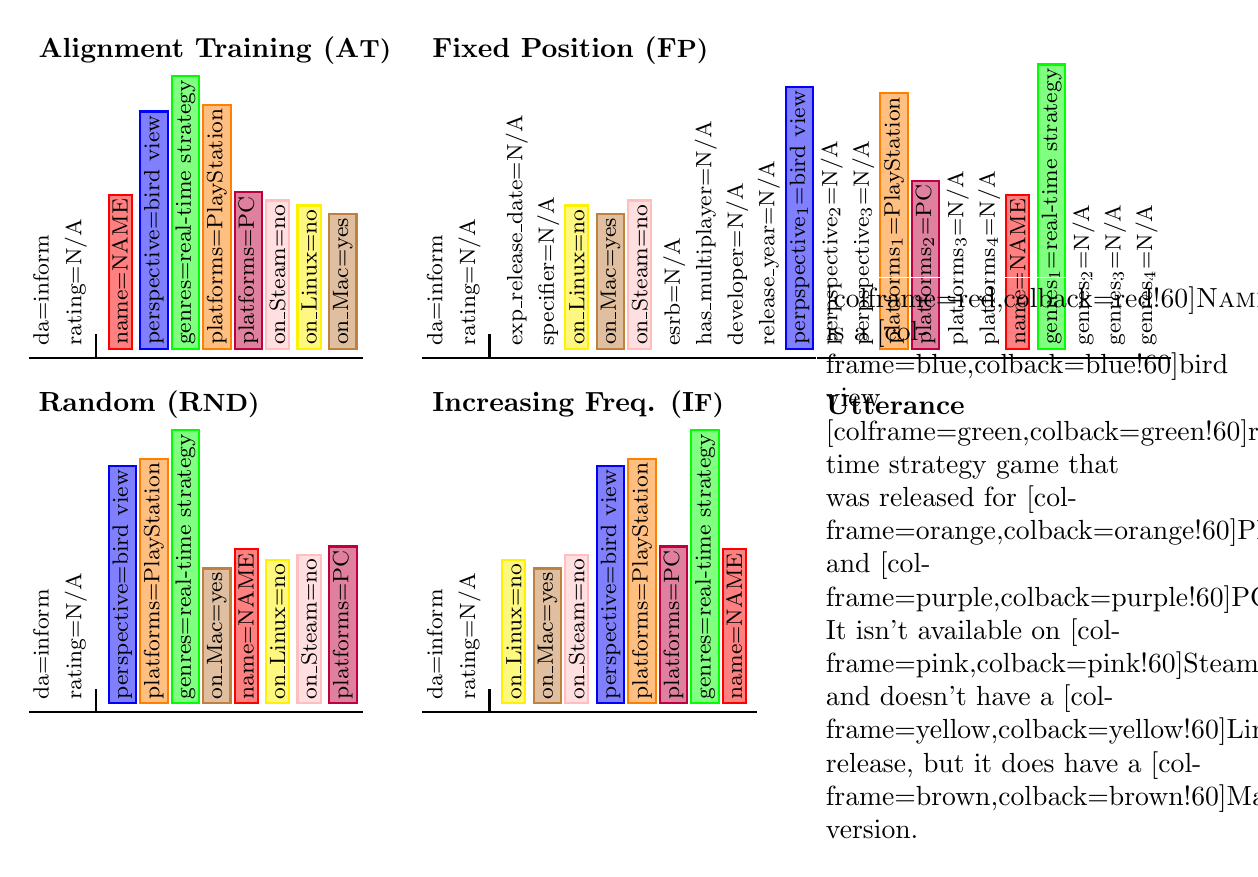
\begin{tikzpicture}[]


    \node[anchor=west] at (5.0,5.8) 
        {\textbf{Fixed Position \textsc{(F\small{P})}}};
    \node[anchor=west] at (0.0,5.8) 
        {\textbf{Alignment Training \textsc{(A\small{T})}}};
    \draw[thick] (0.85,1.9) -- (0.85,2.2);
    \draw[thick] (0,1.9) -- (4.25,1.9);
    \draw[thick] (5 + 0.85,1.9) -- (5 + 0.85,2.2);
    \draw[thick] (5 + 0,1.9) -- (10.25+ 4.25,1.9);
    \draw[thick] (0.85,-2.6) -- (0.85,-2.3);
    \draw[thick] (0,-2.6) -- (4.25,-2.6);
    \draw[thick] (5+0.85,-2.6) -- (5+0.85,-2.3);
    \draw[thick] (5+0,-2.6) -- (5+4.25,-2.6);

    \node[anchor=north west,inner sep=0.5mm,rotate=90] at (0,2) 
        {\footnotesize da=inform};
    \node[anchor=north west,inner sep=0.5mm,rotate=90] at (0.4,2) 
        {\footnotesize rating=N/A};
    \node[anchor=north west,rotate=90,inner sep=0.5mm,draw=red,thick,fill=red!50] 
        at (0.2 + 0.8,2) 
        {\footnotesize name=NAME};
    \node[anchor=north west,rotate=90,inner sep=0.5mm,draw=blue,thick,fill=blue!50] 
        at (0.2 + 1.2,2) {\footnotesize perspective=bird view};
    \node[anchor=north west,rotate=90,inner sep=0.5mm,draw=green,thick,
          fill=green!50] 
        at (0.2 + 1.6,2) {\footnotesize genres=real-time strategy};
    \node[anchor=north west,rotate=90,inner sep=0.5mm,draw=orange,thick,
          fill=orange!50] 
        at (0.2 + 2.0,2) {\footnotesize platforms=PlayStation};
    \node[anchor=north west,rotate=90,inner sep=0.5mm,draw=purple,thick,
          fill=purple!50] 
        at (0.2 + 2.4,2) {\footnotesize platforms=PC};
    \node[anchor=north west,rotate=90,inner sep=0.5mm,draw=pink,thick,
          fill=pink!50] 
        at (0.2 + 2.8,2) {\footnotesize on\_Steam=no};
    \node[anchor=north west,rotate=90,inner sep=0.5mm,draw=yellow,thick,
          fill=yellow!50] 
        at (0.2 + 3.2,2) {\footnotesize on\_Linux=no};
    \node[anchor=north west,rotate=90,inner sep=0.5mm,draw=brown,thick,
          fill=brown!50] 
        at (0.2 + 3.6,2) {\footnotesize on\_Mac=yes};


\node[anchor=north west,inner sep=0.5mm,rotate=90] at (5 + 0,2) 
    {\footnotesize da=inform};
\node[anchor=north west,inner sep=0.5mm,rotate=90] at (5 + 0.4,2) 
    {\footnotesize rating=N/A};
\node[anchor=north west,rotate=90,inner sep=0.5mm] 
    at (5.2 + 0.8,2) 
    {\footnotesize exp\_release\_date=N/A};
\node[anchor=north west,rotate=90,inner sep=0.5mm] 
    at (5.2 + 1.2,2) 
    {\footnotesize specifier=N/A};
\node[anchor=north west,rotate=90,inner sep=0.5mm,draw=yellow,thick,fill=yellow!50] 
    at (5.2 + 1.6,2) 
    {\footnotesize on\_Linux=no};
\node[anchor=north west,rotate=90,inner sep=0.5mm,draw=brown,thick,fill=brown!50] 
    at (5.2 + 2.0,2) 
    {\footnotesize on\_Mac=yes};
\node[anchor=north west,rotate=90,inner sep=0.5mm,draw=pink,thick,fill=pink!50] 
    at (5.2 + 2.4,2) 
    {\footnotesize on\_Steam=no};
\node[anchor=north west,rotate=90,inner sep=0.5mm] 
    at (5.2 + 2.8,2) 
    {\footnotesize esrb=N/A};
\node[anchor=north west,rotate=90,inner sep=0.5mm] 
    at (5.2 + 3.2,2) 
    {\footnotesize has\_multiplayer=N/A};

   % ['inform', 'rating=N/A', 'exp_release_date=N/A', 'specifier=N/A', 'has_linux_release=no', 'has_mac_release=yes', 'available_on_steam=no', 'esrb=N/A', 'has_multiplayer=N/A', 'developer=N/A', 'release_year=N/A', 'player_perspective=bird view', 'player_perspective=N/A', 'player_perspective=N/A', 'platforms=PlayStation', 'platforms=PC', 'platforms=N/A', 'platforms=N/A', 'name=PLACEHOLDER', 'genres=real-time strategy', 'genres=N/A', 'genres=N/A', 'genres=N/A']
\node[anchor=north west,rotate=90,inner sep=0.5mm] 
    at (5.2 + 3.6,2) 
    {\footnotesize developer=N/A};
\node[anchor=north west,rotate=90,inner sep=0.5mm] 
    at (5.2 + 4.0,2) 
    {\footnotesize release\_year=N/A};
\node[anchor=north west,rotate=90,inner sep=0.5mm,draw=blue,thick,fill=blue!50] 
    at (5.2 + 4.4,2) 
    {\footnotesize perpspective\textsubscript{1}=bird view};
\node[anchor=north west,rotate=90,inner sep=0.5mm] 
    at (5.2 + 4.8,2) 
    {\footnotesize perpspective\textsubscript{2}=N/A};
\node[anchor=north west,rotate=90,inner sep=0.5mm] 
    at (5.2 + 5.2,2) 
    {\footnotesize perpspective\textsubscript{3}=N/A};
\node[anchor=north west,rotate=90,inner sep=0.5mm,draw=orange,thick,fill=orange!50] 
    at (5.2 + 5.6,2) 
    {\footnotesize platforms\textsubscript{1}=PlayStation};
\node[anchor=north west,rotate=90,inner sep=0.5mm,draw=purple,thick,fill=purple!50] 
    at (5.2 + 6.0,2) 
    {\footnotesize platforms\textsubscript{2}=PC};
\node[anchor=north west,rotate=90,inner sep=0.5mm] 
    at (5.2 + 6.4,2) 
    {\footnotesize platforms\textsubscript{3}=N/A};
\node[anchor=north west,rotate=90,inner sep=0.5mm] 
    at (5.2 + 6.8,2) 
    {\footnotesize platforms\textsubscript{4}=N/A};
\node[anchor=north west,rotate=90,inner sep=0.5mm,draw=red,thick,fill=red!50] 
    at (5.2 + 7.2,2) 
    {\footnotesize name=NAME};
\node[anchor=north west,rotate=90,inner sep=0.5mm,draw=green,thick,fill=green!50] 
    at (5.2 + 7.6,2) 
    {\footnotesize genres\textsubscript{1}=real-time strategy};
\node[anchor=north west,rotate=90,inner sep=0.5mm] 
    at (5.2 + 8.0,2) 
    {\footnotesize genres\textsubscript{2}=N/A};
\node[anchor=north west,rotate=90,inner sep=0.5mm] 
    at (5.2 + 8.4,2) 
    {\footnotesize genres\textsubscript{3}=N/A};
\node[anchor=north west,rotate=90,inner sep=0.5mm] 
    at (5.2 + 8.8,2) 
    {\footnotesize genres\textsubscript{4}=N/A};


%\node[anchor=north west,rotate=90] at (1.5,2) {genres=platformer};
%\node[anchor=north west,rotate=90] at (2,2) {genres=puzzle};
%\node[anchor=north west,rotate=90] at (2.5,2) {perspective=side vew};
%\node[anchor=north west,rotate=90] at (3,2) {name=NAME};
%\node[anchor=north west,rotate=90] at (3.5,2) {name=NAME};
%\node[anchor=north west,rotate=90] at (4,2) {name=NAME};
%\node[anchor=north west,rotate=90] at (4.5,2) {name=NAME};
%
%
%\node[anchor=north west,rotate=90] at (5.5+0,2) {\small give opinion};
%\node[anchor=north west,rotate=90] at (5.5+0.5,2) {\small rating=good};
%\node[anchor=north west,rotate=90] at (5.5+1,2) {\small genres=adventure};
%\node[anchor=north west,rotate=90] at (5.5+1.5,2) {genres=platformer};
%\node[anchor=north west,rotate=90] at (5.5+2,2) {genres=puzzle};
%\node[anchor=north west,rotate=90] at (5.5+2.5,2) {perspective=side vew};
%\node[anchor=north west,rotate=90] at (5.5+3,2) {name=NAME};
%\node[anchor=north west,rotate=90] at (5.5+3.5,2) {name=NAME};
%\node[anchor=north west,rotate=90] at (5.5+4,2) {name=NAME};
%\node[anchor=north west,rotate=90] at (10+0,2) {give opinion};
%\node[anchor=north west,rotate=90] at (10+0.5,2) {rating=good};
%\node[anchor=north west,rotate=90] at (10+1,2) {genres=adventure};
%\node[anchor=north west,rotate=90] at (10+1.5,2) {genres=platformer};
%\node[anchor=north west,rotate=90] at (10+2,2) {genres=puzzle};
%\node[anchor=north west,rotate=90] at (10+2.5,2) {perspective=side vew};
%\node[anchor=north west,rotate=90] at (10+3,2) {name=NAME};
%\node[anchor=north west,rotate=90] at (10+3.5,2) {name=NAME};
%\node[anchor=north west,rotate=90] at (10+4,2) {name=NAME};
%\node[anchor=north west,rotate=90] at (10+4.5,2) {name=NAME};
%
%



%['give_opinion', 'rating=good', 'genres=adventure', 'genres=platformer', 'genres=puzzle', 'player_perspective=side view', 'name=PLACEHOLDER']


%#
%#

%['inform', 'rating=N/A', 'exp_release_date=N/A', 'specifier=N/A', 'has_linux_release=no', 'has_mac_release=yes', 'available_on_steam=no', 'esrb=N/A', 'has_multiplayer=N/A', 'developer=N/A', 'release_year=N/A', 'player_perspective=bird view', 'player_perspective=N/A', 'player_perspective=N/A', 'platforms=PlayStation', 'platforms=PC', 'platforms=N/A', 'platforms=N/A', 'name=PLACEHOLDER', 'genres=real-time strategy', 'genres=N/A', 'genres=N/A', 'genres=N/A']


%inc_freq_delex
%['inform', 'rating=N/A', 'has_linux_release=no', 'has_mac_release=yes', 'available_on_steam=no', 'player_perspective=bird view', 'platforms=PlayStation', 'platforms=PC', 'name=PLACEHOLDER', 'genres=real-time strategy']

\node[anchor=north west,inner sep=0.5mm,rotate=90] at (0,-2.5) 
    {\footnotesize da=inform};
\node[anchor=north west,inner sep=0.5mm,rotate=90] at (0.4,-2.5) 
    {\footnotesize rating=N/A};
\node[anchor=north west,rotate=90,inner sep=0.5mm,draw=blue,thick,fill=blue!50] 
    at (0.2 + 0.8,-2.5) 
    {\footnotesize perspective=bird view};

\node[anchor=north west,rotate=90,inner sep=0.5mm,draw=orange,thick,fill=orange!50] 
    at (0.2 + 1.2,-2.5) 
    {\footnotesize platforms=PlayStation};
\node[anchor=north west,rotate=90,inner sep=0.5mm,draw=green,thick,fill=green!50] 
    at (0.2 + 1.6,-2.5) 
    {\footnotesize genres=real-time strategy};


\node[anchor=north west,rotate=90,inner sep=0.5mm,draw=brown,thick,fill=brown!50] 
    at (0.2 + 2.0,-2.5) 
    {\footnotesize on\_Mac=yes};
\node[anchor=north west,rotate=90,inner sep=0.5mm,draw=red,thick,fill=red!50] 
    at (0.2 + 2.4,-2.5) 
    {\footnotesize name=NAME};

\node[anchor=north west,rotate=90,inner sep=0.5mm,draw=yellow,thick,fill=yellow!50] 
    at (0.2 + 2.8,-2.5) 
    {\footnotesize on\_Linux=no};
\node[anchor=north west,rotate=90,inner sep=0.5mm,draw=pink,thick,fill=pink!50] 
    at (0.2 + 3.2,-2.5) 
    {\footnotesize on\_Steam=no};
\node[anchor=north west,rotate=90,inner sep=0.5mm,draw=purple,thick,fill=purple!50] 
    at (0.2 + 3.6,-2.5) 
    {\footnotesize platforms=PC};

    \node[anchor=west] at (0,1.3) {\textbf{Random \textsc{(R\small{ND})}}};



\node[anchor=north west,inner sep=0.5mm,rotate=90] at (5 + 0,-2.5) 
    {\footnotesize da=inform};
\node[anchor=north west,inner sep=0.5mm,rotate=90] at (5 + 0.4,-2.5) 
    {\footnotesize rating=N/A};
\node[anchor=north west,rotate=90,inner sep=0.5mm,draw=yellow,thick,fill=yellow!50] 
    at (5.2 + 0.8,-2.5) 
    {\footnotesize on\_Linux=no};
\node[anchor=north west,rotate=90,inner sep=0.5mm,draw=brown,thick,fill=brown!50] 
    at (5.2 + 1.2,-2.5) 
    {\footnotesize on\_Mac=yes};
\node[anchor=north west,rotate=90,inner sep=0.5mm,draw=pink,thick,fill=pink!50] 
    at (5.2 + 1.6,-2.5) 
    {\footnotesize on\_Steam=no};

\node[anchor=north west,rotate=90,inner sep=0.5mm,draw=blue,thick,fill=blue!50]
    at (5.2 + 2.0,-2.5) 
    {\footnotesize perspective=bird view};
\node[anchor=north west,rotate=90,inner sep=0.5mm,draw=orange,thick,fill=orange!50] 
    at (5.2 + 2.4,-2.5) 
    {\footnotesize platforms=PlayStation};
\node[anchor=north west,rotate=90,inner sep=0.5mm,draw=purple,thick,fill=purple!50] 
    at (5.2 + 2.8,-2.5) 
    {\footnotesize platforms=PC};

\node[anchor=north west,rotate=90,inner sep=0.5mm,draw=green,thick,fill=green!50] 
    at (5.2 + 3.2,-2.5) 
    {\footnotesize genres=real-time strategy};
\node[anchor=north west,rotate=90,inner sep=0.5mm,draw=red,thick,fill=red!50] 
    at (5.2 + 3.6,-2.5) 
    {\footnotesize name=NAME};
%has_linux_release=no', 'has_mac_release=yes', 'available_on_steam=no', 'player_perspective=bird view', 'platforms=PlayStation', 'platforms=PC', 'name=PLACEHOLDER', 'genres=real-time strategy'
    \node[anchor=west] at (5.0,1.3) {\textbf{Increasing Freq. \textsc{(I\small{F})}}};


%\node[anchor=north west,inner sep=0.5mm,rotate=90] at (10 + 0,-2.5) 
%    {\footnotesize da=inform};
%\node[anchor=north west,inner sep=0.5mm,rotate=90] at (10 + 0.4,-2.5) 
%    {\footnotesize rating=N/A};
%
%\node[anchor=north west,rotate=90,inner sep=0.5mm,draw=red,thick,fill=red!50] 
%    at (10.2 + 0.8,-2.5) 
%    {\footnotesize name=NAME};
%
%\node[anchor=north west,rotate=90,inner sep=0.5mm,draw=green,thick,fill=green!50] 
%    at (10.2 + 1.2,-2.5) 
%    {\footnotesize genres=real-time strategy};
%
%    \node[anchor=north west,rotate=90,inner sep=0.5mm,draw=purple,thick,fill=purple!50] 
%    at (10.2 + 1.6,-2.5) 
%    {\footnotesize platforms=PC};
%\node[anchor=north west,rotate=90,inner sep=0.5mm,draw=orange,thick,fill=orange!50] 
%    at (10.2 + 2.0,-2.5) 
%    {\footnotesize platforms=PlayStation};
%
%\node[anchor=north west,rotate=90,inner sep=0.5mm,draw=blue,thick,fill=blue!50]
%    at (10.2 + 2.4,-2.5) 
%    {\footnotesize perspective=bird view};
%\node[anchor=north west,rotate=90,inner sep=0.5mm,draw=pink,thick,fill=pink!50] 
%    at (10.2 + 2.8,-2.5) 
%    {\footnotesize on\_Steam=no};
%\node[anchor=north west,rotate=90,inner sep=0.5mm,draw=brown,thick,fill=brown!50] 
%    at (10.2 + 3.2,-2.5) 
%    {\footnotesize on\_Mac=yes};
%\node[anchor=north west,rotate=90,inner sep=0.5mm,draw=yellow,thick,fill=yellow!50] 
%    at (10.2 + 3.6,-2.5) 
%    {\footnotesize on\_Linux=no};
%




%has_linux_release=no', 'has_mac_release=yes', 'available_on_steam=no', 'player_perspective=bird view', 'platforms=PlayStation', 'platforms=PC', 'name=PLACEHOLDER', 'genres=real-time strategy'
%    \node[anchor=west] at (10.0,1.3) {\textbf{Decreasing Freq.}};




    \node[anchor=west] at (10, 1.3) {\textbf{Utterance}};
\node[text width=5.0cm,draw=white,anchor=west] at (10,-0.7) {
    {\mybox[colframe=red,colback=red!60]{\textsc{Name}}} is a 
    \mybox[colframe=blue,colback=blue!60]{bird view} 
    \mybox[colframe=green,colback=green!60]{real-time strategy} 
    game that was released for 
    \mybox[colframe=orange,colback=orange!60]{PlayStation} and 
    \mybox[colframe=purple,colback=purple!60]{PC.} It isn't available on 
    \mybox[colframe=pink,colback=pink!60]{Steam} and doesn't have a 
    \mybox[colframe=yellow,colback=yellow!60]{Linux} release, but it does have
    a \mybox[colframe=brown,colback=brown!60]{Mac} version.
};


\end{tikzpicture}

\caption{Example \meaningrepresentation~linearization strategies for an utterance (lower right) from the 
    ViGGO training set.}
\label{fig:linstrats}
\end{figure}


\paragraph{Increasing Frequency (\textsc{If})} In the \textsc{Increasing
Frequency} linearization (\textsc{If}), we order the attribute-value pairs by
increasing frequency of occurrence in the training data i.e.
$\acount(\attr_i=\aval_i) \le \acount(\attr_{i+1}=\aval_{i+1})$.  We
hypothesize that placing frequently occurring items in a consistent location
may make it easier for the generation model to realize those items correctly,
possibly at the expense of rarer items.

\paragraph{Fixed Position (\textsc{Fp})} We take  consistency one step further
and create a fixed ordering of all attributes, \textit{n.b.} not
attribute-values, ordering them in increasing frequency of occurrence on the
training set (i.e. every instance has the same order of attributes in the
encoder input). In this \textsc{Fixed Position} linearization (\textsc{Fp}),
attributes that are not present in an \meaningrepresentation~are explicitly
represented with an \textit{N/A} value.  For list-valued slots, we determine
the maximum length list in the training data and create that many repeated
slots in the input sequence.  This linearization is feasible for datasets with
a modest number of unique attributes (in our case ViGGO has 14 attributes and
the E2E Challenge corpus has eight) but would not easily scale to 10s, 100s, or
larger attribute vocabularies. 

\subsection{Phrase-based Data Augmentation}
\label{sec:pbda}

\begin{figure}
    \centering


        \begin{tikzpicture}

            \def\th{5mm};
            \def\td{2mm};
    \node[text height=\th,text depth=\td] (aromi) at (-5,-4) {Aromi};
            \node[text height=\th,text depth=\td] (is) at (-1.5,-4) {is};
            \node[text height=\th,text depth=\td] (not) at (0.0,-4) {not};

            \node[text height=\th,text depth=\td] (a) at (1.5,-4) {a};
            \node[text height=\th,text depth=\td] (ff) at (4,-4) {family-friendly};
            \node[text height=\th,text depth=\td] (est) at (6.5,-4) {establishment};


            \node (root) at (-2.5,0) {S};
            \node[draw,circle,font=\small,inner sep=0] at ($(root)+(-0.5,0.5)$) {4};
            \node (rootNP) at (-5,-1) {NP};
            \node[draw,circle,font=\small,inner sep=0] at ($(rootNP)+(-0.5,0.5)$) {3};
            \node (rootNPNNP) at (-5,-2) {NNP};
            \node (r1c2) at (0.0,-1) {VP};
            \node[draw,circle,font=\small,inner sep=0] at ($(r1c2)+(0.5,0.5)$) {2};
                \node (r2c3) at (4,-2) {NP};
            \node[draw,circle,font=\small,inner sep=0] at ($(r2c3)+(0.5,0.5)$) {1};
                \node (det) at (1.5,-3) {DET};
                \node (jj) at (4,-3) {JJ};
                \node (nn) at (6.5,-3) {NN};
                \node (r2c1) at (-1.5,-2) {VB};

                \node (r2c2) at (0.0,-2) {RB};
                \draw[-] (r1c2) -- (r2c1);
                \draw[-] (r1c2) -- (r2c2);
                \draw[-] (r1c2) -- (r2c3);


                \draw[-] (r2c1) -- (is);

            \draw[-] (rootNPNNP) -- (aromi);
            \draw[-] (root.south west) -- (rootNP.north east);
            \draw[-] (rootNP) -- (rootNPNNP);
            \draw[-] (root.south east) -- (r1c2.north west);
                \draw[-] (r2c3) -- (det);
                \draw[-] (r2c3) -- (jj);
                \draw[-] (r2c3) -- (nn);
                \draw[-] (det) -- (a);
                \draw[-] (jj) -- (ff);
                \draw[-] (nn) -- (est);
                \draw[-] (r2c2) -- (not);
        

      %      \node[anchor=north west,align=left,inner sep=0,outer sep=0,text height=0mm,text width=11cm] at (0.7,0.5) {
                    %\begin{enumerate}
                    %    \item Parse training examples.
                %\item<3-> Create additional training examples from constituent phrases.
                %\end{enumerate}};

        \end{tikzpicture}

        ~\\~\\

        \begin{tabular}{ccc}
            \toprule
            &         \MeaningRepresentation~($\mr$) & Utterance ($\utttoks$) \\
            \midrule
            \raisebox{0.5pt}{\textcircled{\raisebox{-0.9pt} {1}}} &  
        $\left[\!\!\left[ \begin{array}{l} 
            \textsc{Inform}\\ 
            \AV{family\_friendly}{yes} 
        \end{array}   \right]\!\!\right]$  & 
            $\left[\textit{<<s>>}, \textit{a}, \textit{family-friendly}, \textit{establishment}, \textit{<<e>>}\right]$\\
        \raisebox{0.5pt}{\textcircled{\raisebox{-0.9pt} {2}}} &
        $\left[\!\!\left[ \begin{array}{l} 
            \textsc{Inform}\\ 
            \AV{family\_friendly}{no} 
        \end{array}\right]\!\!\right]$  & 
            $\left[\textit{<<s>>}, \textit{is}, \textit{not}, \textit{a}, 
            \textit{family-friendly}, \textit{establishment}, \textit{<<e>>}\right]$ \\
        \raisebox{0.5pt}{\textcircled{\raisebox{-0.9pt} {3}}} &
        $\left[\!\!\left[ \begin{array}{l} 
            \textsc{Inform}\\ 
            \AV{name}{Aromi} \end{array}   
        \right]\!\!\right]$ &  
        $\left[\textit{<<s>>}, \textit{aromi}, \textit{<<e>>}\right]$ \\
        \raisebox{0.5pt}{\textcircled{\raisebox{-0.9pt} {4}}} &
        $\left[\!\!\left[ \begin{array}{l}
            \textsc{Inform}\\ 
            \AV{name}{Aromi} \\ 
            \AV{family\_friendly}{no} 
        \end{array}\right]\!\!\right]$  & 
        $\left[\textit{<<s>>}, \textit{aromi}, \textit{is}, \textit{not}, 
               \textit{a}, \textit{family-friendly}, \textit{establishment}, 
               \textit{<<e>>}\right]$ \\
        \bottomrule
        \end{tabular}
    \caption{Example training instances produced from the phrase-based
            data augmentation protocol. The constituent parse is shown
        above. Numbered phrase nodes correspond to the phrase examples
    created in the table below.}
            \label{fig:pbdaexample}
\end{figure}


While the alignment training linearization induces control in a
\sequencetosequence~model, the resulting model will still likely have trouble
following utterance plans that are not well represented in the training data.
As we discussed in \autoref{sec:nlgfg}, \sequencetosequence~models do not seem
understand the compositional nature of phrase structure in language data. With
this problem in mind, we propose a phrase-based data-augmentation method for
creating additional training examples from constituent phrases of the training
data. In doing so, we directly expose the model to instances of syntactic
composition, and how that composition systematically changes the semantics of
the utterance.

We parse all training utterances and create additional training utterances from
constituent phrases governed by NP, VP, ADJP, ADVP, PP, S, Sbar
non-terminals.\footnote{We used the
\href{https://stanfordnlp.github.io/CoreNLP/}{Stanford CoreNLP parser v3.9.2}.}
Because a phrase may mean something different than the larger utterance it is
embedded in, we apply the utterance tagger used for alignment training (see
\autoref{sec:align}) to obtain the correct attribute-values denoted by the
phrase. Since the tagger does not predict the dialogue act, we assign the
dialogue act of the original training utterance to the new phrase's meaning
representation.  If a new phrase example obtained by this process does not have
any attribute predicted by the tagger, we discard it.

Because we reclassify the \meaningrepresentation~of phrases using the utterance
tagger, the augmented  data includes examples of how to negate binary
attributes.  See for example in \autoref{fig:pbdaexample} where we extract the
noun phrase ``a family-friendly establishment'' which implies
\textit{family\_friendly=yes} and its composition with a verb phrase ``is
not'', which changes the meaning to \textit{family\_friendly=no}.

When presenting the linearized \meaningrepresentation of phrase examples to the
model encoder we prepend and append phrase specific start and stop tokens
respectively (e.g., \textit{<<s-NP>>} and \textit{<<e-NP>>}) to prevent the
model from ever producing an incomplete sentence when generating for a complete
\meaningrepresentation.

\subsection{Datasets}

We run our alignment training experiments on the E2E Challenge dataset as well
as the more recently released ViGGO corpus \citep{juraska2019} another English
language, task-oriented dialogue
dataset.\footnote{\url{https://nlds.soe.ucsc.edu/viggo}} The ViGGO corpus comes
from the video game domain (i.e., conversations with a video game
recommendation agent)  and  contains 14 attribute types and nine dialogue acts.
In addition to binary and categorical valued attributes, the corpus also
features list-valued attributes which can have a variable number of values, and
an open-class \Atr{specifier} attribute. 

\subsubsection{Meaning Representation/Utterance Alignments} \label{sec:align}

The original datasets do not have alignments between individual attribute-value
pairs and the subsequences of the utterances they occur in, which we need for
the alignment training linearization strategy.  We manually developed a list of
heuristic pattern matching rules (e.g., ``not kid-friendly'' $\rightarrow$
\textit{family\_friendly=no}) which we use to tag the utterance tokens.  For
ViGGO, we started from scratch, but for the E2E Challenge dataset we greatly
expanded the rule-set created by \citet{dusek2019}.  To ensure the correctness
of the rules, we iteratively added new matching rules, ran them on the training
and validation sets, and verified that they produced the same
\meaningrepresentation~as was provided in the dataset. This process took the
author roughly two weeks to produce approximately 25,000 and 1,500 rules for
the E2E and ViGGO datasets respectively. Note that the large number of rules is
obtained programmatically, i.e. creating template rules and inserting matching
keywords or phrases (e.g., enumerating variants such as \textit{not
kid-friendly}, \textit{not child-friendly}, \textit{not family-friendly},
etc.).

\begin{table}
\centering
\begin{tabular}{cc cccc}
\toprule
Dataset & Train & Augmented & Valid & Test \\
\midrule
E2E Challenge & 33,523 & 443,192 & 4,299  & 4,693 \\
ViGGO         &  5,103 &  67,445 & 714 & 1,083 \\
% contains 5,103 train/246 dev/359 test)
\bottomrule
\end{tabular}
\caption{Dataset sizes (including data augmentation) after correcting
the training and validation instances.}
\label{tab:cgdata}
\end{table}


In cases where the matching rules produced different
\meaningrepresentations~than provided in the original dataset, we manually
checked them. If the rule was incorrect, we added a new rule to account for the
exception.  In many cases in the E2E Challenge dataset and several times in the
ViGGO corpus, we found the rule to be correct and the \meaningrepresentation~to
be incorrect for the given utterance. In those cases, we used the corrected
\meaningrepresentations~for training and validation.  We do not modify the test
sets in any way. We follow \citet{dusek2019} and remove from the training and
validation sets any modified examples that share a \meaningrepresentation~also
found in the test set. This creates slightly different training and validation
set numbers for the E2E Challenge dataset than in the faithful generation
experiments. See \autoref{tab:cgdata} for statistics.  We use the matching
rules to develop  a rule-based utterance tagger to implement the alignment
training linearization, phrase-based data augmentation protocol, and as a
reranker when generating utterances in our experiments.

For most cases, the attribute-values uniquely correspond to a non-overlapping
subsequences of the utterance. The \Atr{\textit{rating}} attribute in the ViGGO
dataset, however, could have multiple reasonable mappings to the utterance, so
we treat it in practice like an addendum to the dialogue act, occurring
directly after the dialogue act as part of a ``header'' section in any
\meaningrepresentation~linearization strategy (see \autoref{fig:linstrats}
where \textit{rating=N/A} occurs after the dialogue act regardless of choice of
linearization strategy).

\paragraph{Delexicalization} The ViGGO corpus is relatively small and the
attributes \Atr{name}, \Atr{developer}, \Atr{release\_year},
\Atr{expected\_release\_date}, and \Atr{specifier}~can have values that are
only seen several times during training. Neural models often struggle to learn
good representations for infrequent inputs, which can, in turn, lead to poor
test-set generalization. To alleviate this, we delexicalize these values in the
utterance. That is, we replace them with an attribute specific placeholder
token.

\label{app:specifier} Additionally, for \Atr{specifier} whose values come from
the open class of adjectives, we represent the specified adjective with a
placeholder which marks two features, whether it is consonant (C) or vowel
initial (V) (e.g.  ``\uline{d}ull'' vs. ``\uline{o}ld'') and whether it is in
regular (R) or superlative (S) form (e.g. ``dull'' vs. ``dullest'') since these
features can effect the surrounding context in which the adjective is realized.
See the following lexicalized/delexicalized examples:
\begin{itemize}
        \item \AV{specifier}{oldest}~-- vowel initial, superlative
\begin{itemize}
    \item \textit{What is the oldest game you've played?}
    \item \textit{What is the SPECIFIER\_V\_S game you've played?}
\end{itemize}
        \item \AV{specifier}{old}~-- vowel initial, regular

\begin{itemize}
    \item \textit{What is an old game you've played?}
    \item \textit{What is an SPECIFIER\_V\_R game you've played?}
\end{itemize}

        \item \AV{specifier}{new}~-- consonant initial, regular

\begin{itemize}
    \item \textit{What is a new game you've played?}
    \item \textit{What is a SPECIFIER\_C\_R game you've played?}
\end{itemize}
\end{itemize}
Under this delexicalization scheme, models can learn the appropriate articles
(if any) to use before realizing a particular specifier value.

All generated delexicalized utterances are post-processed with the
corresponding attribute-values before computing evaluation metrics (i.e., they
are re-lexicalized with the appropriate value strings from the input
\meaningrepresentation). Unlike in the faithful generation experiments, we do
not perform any delexicalization of the E2E Challenge corpus.

\subsection{Generation Models}

We examine the effects of linearization strategy and data augmentation on biGRU
(see \autoref{sec:nlggru}) and transformer (see \autoref{sec:nlgtf}) based
\sequencetosequence~models.  See \autoref{tab:nlghpsspace} for the set of
hyper-parameters that we explored for each model and \autoref{tab:gruparams}
and \autoref{tab:tfparams} for the winning hyper-parameter settings for the
biGRU and transformer models respectively.  Hyper-parameters were found using
grid-search, selecting the model with best validation \textsc{Bleu} score. We
performed a separate grid-search for each architecture-linearization strategy
pairing in case there was no one best hyper-parameter setting.  We used a batch
size of 128 for all biGRU and Transformer models and trained for at most 700
epochs.

\begin{table}
    \centering
    \begin{tabular}{cp{4.25cm}p{4.25cm}}
            \toprule
            Hyperparameter & biGRU & Transformer\\
            \midrule
            Layers & $1$, $2$ & $1$, $2$\\
            Label Smoothing & $0.0$, $0.1$ & $0.0$, $0.1$\\
            Weight Decay & $0$, $10^-5$ & --- \\
Optimizer/Learning Rate & Adam/$10^{-3}$, Adam/$10^{-4}$, Adam/$10^{-5}$,
            SGD/$0.5$, SGD/$0.25$, SGD/$0.1$ & Adam with the learning
            rate schedule from \cite{rush2018} (factor=1, warmup=8000)\\
        Tied Decoder Embeddings & tied, untied & tied, untied\\
        Attention & Bahdanau, General & ---\\
        \bottomrule
\end{tabular}
\caption{Hyperparameter search space for biGRU and transformer architectures.}
\label{tab:nlghpsspace}
\end{table}


\begin{table}
\small
\center
\begin{tabular}{clccc ccc cc ccccc}
\toprule
&Model & L & LS & WD & Optim. & LR & Attn & $\embDim$ & $\hidDim$ & $\encDim$ & $\decDim$ & Drop. & Params \\
\midrule
    \parbox[t]{2mm}{\multirow{6}{*}{\rotatebox[origin=c]{90}{E2E}}} 
 & \textsc{Rnd} & 2 & 0.1 & $10^{-5}$ & Adam & $10^{-5}$ &  Bahd. & 512 & 512 & 1024 & 512 & 0.1 & 14,820,419  \\
 & \textsc{Fp} & 2 & 0.1 & $10^{-5}$ & SGD & $0.1$ &  Bahd. & 512 & 512 & 1024 & 512 & 0.1 & 14,820,003 \\ 
 & \textsc{If} & 2 & 0.1 & $0.0$ & SGD & $0.5$ &  Gen. & 512 & 512 & 1024 & 512  & 0.1 & 14,557,763 \\
 & \textsc{If+p} & 2 & 0.1 & $0.0$ & SGD & $0.5$ &  Gen. &512 & 512 & 1024 & 512  & 0.1 &14,557,763 \\
 & \textsc{At} & 2 & 0.1 & $10^{-5}$ & Adam & $10^{-5}$ &  Bahd. & 512 & 512 & 1024 & 512  & 0.1 & 14,820,419  \\
 & \textsc{At+p} & 2 & 0.1 & $10^{-5}$ & Adam & $10^{-5}$ &  Bahd. & 512 & 512 & 1024 & 512  & 0.1 & 14,820,419  \\
\midrule
    \parbox[t]{2mm}{\multirow{6}{*}{\rotatebox[origin=c]{90}{ViGGO}}} 
 & \textsc{Rnd} & 2 & 0.1 & $10^{-5}$ & SGD & $0.25$ &  Gen. & 512 & 512 & 1024 & 512 & 0.1 & 14,274,865 \\
 & \textsc{Fp} & 1 & 0.1 & $10^{-5}$ & Adam & $10^{-5}$ &  Bahd. & 512 & 512 & 1024 & 512 & 0.1 & 7,718,193 \\ 
 & \textsc{If} & 1 & 0.0 & $0.0$ & SGD & $0.5$ &  Bahd. &  512 & 512 & 1024 & 512  & 0.1 & 7,712,049 \\ 
 & \textsc{If+} & 1 & 0.0 & $0.0$ & SGD & $0.5$ &  Bahd. & 512 & 512 & 1024 & 512  & 0.1 & 7,712,049 \\ 
 & \textsc{At} & 2 & 0.1 & $0.0$ & Adam & $10^{-5}$ &  Bahd. &  512 & 512 & 1024 & 512  & 0.1 & 14,537,521 \\ 
 & \textsc{At+p} & 2 & 0.1 & $0.0$ & Adam & $10^{-5}$ &  Bahd. &  512 & 512 & 1024 & 512  & 0.1 & 14,537,521 \\ 
\bottomrule
\end{tabular}

\caption{Winning hyperparameter settings for biGRU models. L, LS, and WD 
indicate number of layers, label smoothing, and weight decay respectively. 
All models use untied embeddings. Drop. indicates dropout (i.e. drop probability).}
\label{tab:gruparams}
\end{table}

\begin{table}
\center
\begin{tabular}{cl cccc ccccc}
\toprule
&Model & Layers & LS & Emb. & Params & $\embDim$ & $\hidDim$ & $\encDim$ & $\decDim$ & Dropout\\
\midrule
    \parbox[t]{2mm}{\multirow{6}{*}{\rotatebox[origin=c]{90}{E2E}}} 
 & \textsc{Rnd} & 1 & 0.1 & tied & 7,966,787 & 512 & 2048 & 512 & 512 & 0.1\\
 & \textsc{Fp} & 1 & 0.1 & tied & 7,970,371 & 512 & 2048 & 512 & 512 & 0.1\\
 & \textsc{If} & 1 & 0.1 & untied & 8,525,379 & 512 & 2048 & 512 & 512 & 0.1 \\
 & \textsc{If+p} & 1 & 0.1 & untied & 8,525,379 & 512 & 2048 & 512 & 512 & 0.1 \\
 & \textsc{At} & 2 & 0.1 & untied & 15,881,795 & 512 & 2048 & 512 & 512 & 0.1 \\
 & \textsc{At+p} & 2 & 0.1 & untied & 15,881,795 & 512 & 2048 & 512 & 512 & 0.1 \\
\midrule
    \parbox[t]{2mm}{\multirow{6}{*}{\rotatebox[origin=c]{90}{ViGGO}}} 
 & \textsc{Rnd} & 2 & 0.0 & untied & 15,598,897 & 512 & 2048 & 512 & 512 & 0.1\\
 & \textsc{Fp} & 2 & 0.1 & untied & 15,605,041 & 512 & 2048 & 512 & 512 & 0.1\\
 & \textsc{If} & 2 & 0.1 & untied & 15,598,897 & 512 & 2048 & 512 & 512 & 0.1 \\
 & \textsc{If+p} & 2 & 0.1 & untied & 15,598,897 & 512 & 2048 & 512 & 512 & 0.1\\
 & \textsc{At} & 2 & 0.1 & untied & 15,598,897 & 512 & 2048 & 512 & 512 & 0.1 \\
 & \textsc{At+p} & 2 & 0.1 & untied & 15,598,897 & 512 & 2048 & 512 & 512 & 0.1 \\
\bottomrule
\end{tabular}

\caption{Winning hyperparameter settings for transformer models 
(trained from scratch). L and  LS indicate number of layers and label smoothing respectively. Drop. indicates dropout (i.e. drop probability).
All models trained with the Adam optimizir with the learning
            rate schedule from \cite{rush2018} (factor=1, warmup=8000).
}
\label{tab:tfparams}
\end{table}


\newcommand{\utt}{\ensuremath{\mathbf{y}}}
\newcommand{\uttVocab}{\ensuremath{\mathcal{W}}}
\newcommand{\da}{\ensuremath{a}}
\newcommand{\inseq}{\mathbf{x}}
\newcommand{\Attrs}{\ensuremath{\mathcal{V}}}
\newcommand{\inSize}{m}
\newcommand{\outSize}{n}

\newcommand{\mmhAttn}{\operatorname{maskedMHAttn}}
\newcommand{\mhAttn}{\operatorname{MHAttn}}

\newcommand{\mrEmb}{\mathbf{W}}
\newcommand{\uttEmb}{\mathbf{V}}
\newcommand{\decInput}{\mathbf{G}}
\newcommand{\decInputi}{\mathbf{g}_i}


\newcommand{\tfeA}{\boldsymbol{\check{\encInput}}^{(i)}}
\newcommand{\tfeB}{\boldsymbol{\bar{\encInput}}^{(i)}}
\newcommand{\tfeC}{\boldsymbol{\hat{\encInput}}^{(i)}}
\newcommand{\tfeD}{\boldsymbol{\dot{\encInput}}^{(i)}}
\newcommand{\tfeE}{\boldsymbol{\ddot{\encInput}}^{(i)}}

\newcommand{\tfdA}{\boldsymbol{\check{\decInput}}^{(i)}}
\newcommand{\tfdB}{\boldsymbol{\bar{\decInput}}^{(i)}}
\newcommand{\tfdC}{\boldsymbol{\hat{\decInput}}^{(i)}}
\newcommand{\tfdD}{\boldsymbol{\grave{\decInput}}^{(i)}}
\newcommand{\tfdE}{\boldsymbol{\tilde{\decInput}}^{(i)}}
\newcommand{\tfdF}{\boldsymbol{\acute{\decInput}}^{(i)}}
\newcommand{\tfdG}{\boldsymbol{\dot{\decInput}}^{(i)}}
\newcommand{\tfdH}{\boldsymbol{\ddot{\decInput}}^{(i)}}

Additionally, we fine-tune BART \cite{lewis2020}, a large, pretrained
transformer-based \sequencetosequence~model. We stop fine-tuning after
validation set cross-entropy stops decreasing.  We use the same settings as the
fine-tuning for the CNN-DailyMail summarization task, although we modify the
maximum number of updates to be roughly to be equivalent to 10 epochs on the
training set when using a 500 token batch size, since the number of updates
effects the learning rate scheduler. We selected the model iterate with lowest
validation set cross-entropy.

While BART is unlikely to have seen any linearized MR in its pretraining data,
its use of sub-word encoding  allows it to encode arbitrary strings. Rather
than extending it's encoder input vocabulary to add the MR tokens, we simply
format the input MR as a string (in the corresponding linearization order),
e.g. ``inform rating=good name=NAME platforms=PC platforms=Xbox''.

\subsection{Utterance Planner Model} We experiment with three approaches to
creating a test-time utterance plan for the alignment training models. The
first is a bigram language model (\BgUP) over attribute-value sequences.
Attribute-value bigram counts are estimated from the training data (using
Lidstone smoothing \citep{chen1996} with $\lidstone=10^{-6}$)  according to the
ordering determined by the matching rules (i.e. the alignment-training
ordering). 

\begin{table}
\centering
\begin{tabular}{cc}
\toprule
Hyperparameter & Search Space\\
\midrule
Layers & 1, 2\\
Learning Rate &$10^{-3}$, $10^{-4}$, $10^{-5}$\\
RNN Cell & GRU, LSTM \\
Encoder direction & uni-, bi- \\
Label Smoothing & 0.0, 0.1\\
\bottomrule
\end{tabular}
\caption{Hyperparameter search space for the neural utterance planner (NUP).}
\label{tab:nuphps}
\end{table}


\begin{table}
\centering
\begin{tabular}{c ccc ccc ccccc}
\toprule
Dataset & L & Enc. Dir. & RNN Cell& LR & LS & Attn. &$\embDim$ & $\hidDim$  & $\encDim$ & $\decDim$ & Dropout \\
\midrule
   E2E & 1 & bi- &LSTM& $10^{-5}$ & 0.1 & Bahd. & 512 & 512 & 1024 & 512 & 0.1\\
ViGGO & 1 & uni- & LSTM & $10^{-4}$ & 0.1 & Bahd.  & 512 & 512 & 1024 & 512 & 0.1\\ 
\bottomrule
\end{tabular}
\caption{Winning hyperparameter options for the neural utterance planner (NUP)
model.}
\label{tab:nuphp}
\end{table}


The second model is a recurrent neural network based \sequencetosequence~model,
which we refer to as the neural utterance planner (\NUP). We train the \NUP~to
map \textsc{If} ordered attribute-values to the alignment training ordering. We
grid-search model hyperparameters, selecting the model with highest average
Kendall's $\tau$ \citep{kendall1938} on the validation set alignment training
orderings. See \autoref{tab:nuphps} for the hyperparameter search space and
\autoref{tab:nuphp} to see the chosen hyperparameter setting. We used a batch
size of 128, the Adam optimizer, and trained for at most 50 epochs.   Unlike
the \BgUP~model, the \NUP~model also conditions on the dialogue act, so it can
learn ordering preferences that differ across dialogue acts.

For both \BgUP~and \NUP, we use beam search (with beam size 32) to generate
candidate utterance plans. The beam search is constrained to only generate
attribute-value pairs that are given in the supplied \meaningrepresentation,
and to avoid generating repeated attributes. The search is not allowed to
terminate until all attribute-values in the \meaningrepresentation~are
generated.  Beam candidates are ranked by log likelihood. We show validation
and test set Kendall's $\tau$ to the reference utterance for both planning
models in \autoref{tab:uptau}.  A Kendall's $\tau$ of 1.0 indicates that the
planner exactly follows the human reference order while 0.0 indicates a random
order relative to the human reference. $\tau=-1$ indicates the model produces
the reverse order of the human reference plan. We see that the NUP produces
utterance plans that are closer in order to the human reference on both the E2E
Challenge and ViGGO datasets.

\begin{table}
\centering

\begin{tabular}{ll c c}
\toprule
Dataset & Model & Valid & Test \\
\midrule
ViGGO & \textsc{BgUP} & 0.417 & 0.347 \\
                       & \textsc{NUP} & 0.739 & 0.651 \\
\midrule
E2E & \textsc{BgUP} & 0.433 & 0.432 \\
                       & \textsc{NUP} & 0.502 & 0.447 \\
\bottomrule
\end{tabular}


\caption{Validation and test set Kendall's $\tau$ for \textsc{BgUP} and 
NUP models.}
\label{tab:uptau}
\end{table}


The final ordering we propose is the \Oracle~ordering, i.e. the utterance plan
implied by the human-authored test-set reference utterances. This plan
represents the model performance if it had a priori knowledge of the reference
utterance plan. When a test example has multiple references, we select the most
frequent ordering in the references, breaking ties according to
\BgUP~log-likelihood.

\subsection{Experiments}

\subsubsection{Test-Set Evaluation}

In our first experiment, we compare performance of the proposed models and
linearization strategies on the E2E Challenge and ViGGO test sets.  We refer to
models using the alignment training linearization strategy as \textsc{At+BgUP},
\textsc{At+NUP}, or \textsc{At+Oracle} depending on whether the model is
following the bigram planner, neural planner, or human reference plan
respectively.  For the \textsc{If} and \textsc{At+NUP} models we also include
variants trained on the union of original training data and phrase-augmented
data (see \autoref{sec:pbda}), which we denote \textsc{+p}.

\paragraph{Evaluation Measures} For automatic quality measures, we report
\bleu~and \rougel  scores using the official E2E Challenge evaluation
script.\footnote{\url{https://github.com/tuetschek/e2e-metrics}} Additionally,
we use the rule-based utterance tagger to automatically annotate the
attribute-value spans of the model generated utterances, and then manually
verify/correct them. With the attribute-value annotations in hand we compute
the number of missing, wrong, or added attribute-values for each model. From
these counts, we compute the semantic error rate (SER) \citep{dusek2020} where
\[ \textrm{SER} = \frac{\#missing + \#wrong + \#added}{\#attributes}.\]  On
ViGGO, we do not include the \Atr{rating} attribute in this evaluation since we
consider it part of the dialogue act.  Additionally, for \textsc{At} variants,
we report the order accuracy (OA) as the percentage of generated utterances
that correctly follow the provided utterance plan. Utterances with wrong or
added attribute values are counted as not following the utterance plan. 

All models are trained five times with different random seeds; we report the
mean of all five runs. We report statistical significance using Welch's
$t$-test \citep{welch1947}, comparing the score distribution of the five runs
from the best linearization strategy against all other strategies at the $0.05$
level.

\paragraph{Baselines} On the ViGGO dataset we compare to the transformer
baseline of \citet{juraska2019}, which used a beam search of size 10 and
heuristic attribute reranker (similar to our attribute-value matching rules).
On the E2E Challenge dataset, we report the results of TGen+ \citep{dusek2019},
an LSTM-based \sequencetosequence~model, which also uses beam search with a
matching rule based reranker to select the most semantically correct utterance
and is trained on a cleaned version of the corpus (similar to our approach).
 
\subsubsection{Random Permutation Stress Test}

Differences between an \textsc{At} model following an utterance planner model
and the human oracle are often small so we do not learn much about the limits
of controllability of such models, or how they behave in extreme conditions
(i.e. on an arbitrary, random utterance plan, not drawn from the training data
distribution). In order to perform such an experiment we generate random
utterance plans (i.e. permutations of attribute-values) and have the
\textsc{At} models generate utterances for them, which we evaluate with respect
to SER and OA (we lack ground truth references with which to evaluate \bleu~or
\rougel).  We generate random permutations of size $3,4,\ldots, 8$ on the E2E
dataset, since there are 8 unique attributes on the E2E dataset. For ViGGO we
generate permutations of size $3,4,\ldots,10$ (96\% of the ViGGO training
examples fall within this range). For each size we generated 100 random
permutations and all generated plans were given the \textsc{Inform} dialogue
act. In addition to running the \textsc{At} models on these random
permutations, we also compare them to the same model after using the NUP  to
reorder them into an easier\footnote{Easier in the sense that the
\NUP~re-ordering is closer to the training set distribution of \textsc{At}
utterance plans.} ordering.

\subsubsection{Human Evaluation} In our final experiment, we had human
evaluators rank the 100 outputs of the size 5 random permutations for three
\BART~models on both datasets: (i) \textsc{At+p} model with \NUP,  (ii)
\textsc{At+p} model, and (iii) \textsc{At} model.  The first model, which uses
an utterance planner, is likely to be more natural since it doesn't have to
follow the random order, so it serves as a ceiling.  The second and third
models will try to follow the random permutation ordering, and are more likely
to produce unnatural transitions between awkward sequences of attribute-values.
Differences between these models will allow us to understand how the
phrase-augmented data affects the fluency of the models.  The annotators were
asked to rank outputs by their naturalness/fluency.  Each set was annotated
twice by different annotators so we can compute agreement. 

\newcommand{\lsname}[1]{\textsc{#1}}
\newcommand{\lsshort}[1]{\textsc{#1}}
\newcommand{\size}[1]{|#1|}
\newcommand{\lin}{\pi}
\newcommand{\valstr}[1]{\textit{#1}}
\newcommand{\uttstr}[1]{\textit{#1}}
\newcommand{\alignshort}{AT}
\newcommand{\enc}{Enc}
\newcommand{\rep}{h}
\newcommand{\attrval}[2]{#1=#2}
\newcommand{\phraseAug}{+p}
\newcommand{\DA}[1]{\textsc{#1}}

\subsection{Results}

\paragraph{\lsshort{At} models accurately follow utterance plans.} See
\autoref{tab:main.e2e.test} and \autoref{tab:main.viggo.test} for results on
E2E Challenge and ViGGO test sets respectively.  The best non-\Oracle~results
are show in bold for each model and results that are not different with
statistical significance to the best results are underlined.  We see that the
\lsshort{At+NUP} strategy consistently receives the lowest semantic error rate
and highest order accuracy, regardless of architecture or dataset, suggesting
that alleviating the model's decoder of content planning is highly beneficial
to avoiding errors. The Transformer \lsshort{At} model is able to consistently
achieve virtually zero semantic error on the E2E Challenge dataset using either
the bigram or neural planner model.

We also see that fine-tuned BART is able to learn to follow an utterance plan
as well. When following the neural utterance planner, BART is highly
competitive with the trained from scratch Transformer on the E2E Challenge
dataset and surpassing it on the ViGGO dataset in terms of semantic error rate.

\begin{table}[p]
    \centering
    \begin{minipage}[t]{0.45\linewidth}
    \resizebox{\linewidth}{!}{
    \begin{tabular}{ll cccc}
    \toprule
    \multicolumn{2}{c}{Model}&B$\uparrow$&R$\uparrow$&SER$\downarrow$&OA$\uparrow$    \\
    \midrule
    \multicolumn{2}{c}{TGen+} & \multirow{2}{*}{66.0} & \multirow{2}{*}{67.6} &
    \multirow{2}{*}{0.03} & \multirow{2}{*}{---}\\
    \multicolumn{2}{c}{\footnotesize \cite{dusek2019}} & \\
    \midrule
    \parbox[t]{2mm}{\multirow{8}{*}{\rotatebox[origin=c]{90}{biGRU}}}
     & \lsshort{Rnd}  & \textbf{66.8} & 68.3 & 2.64 & --- \\
     & \lsshort{Fp}  & \uline{63.4} & \uline{65.6} & \uline{6.54} & --- \\
     & \lsshort{If}  & 59.2 & 62.7 & 12.64 & --- \\
     & \lsshort{If{\small+p}}  & 65.8 & 68.1 & 0.24 & --- \\
     & \lsshort{At\small{+BgUP}}  & \uline{66.4} & 68.3 & 0.26 & 98.2 \\
     & \lsshort{At\small{+NUP}}  & \uline{66.3} & 68.9 & 0.26 & 98.3 \\
     & \lsshort{At\small{+NUP+p}}  & \uline{66.5} & \textbf{69.1} & \textbf{0.00} & \textbf{100.0} \\
     & \lsshort{At \small{Oracle}}  & 69.8 & 77.3 & 0.84 & 94.3 \\
    \midrule
    \parbox[t]{2mm}{\multirow{8}{*}{\rotatebox[origin=c]{90}{Transformer}}}
     & \lsshort{Rnd}  & \textbf{67.4} & 68.2 & \uline{1.06} & --- \\
     & \lsshort{Fp}  & \textbf{67.4} & \uline{68.7} & \uline{3.10} & --- \\
     & \lsshort{If}  & \uline{67.1} & 68.1 & \uline{0.66} & --- \\
     & \lsshort{If\small{+p}}  & \uline{66.8} & 68.3 & \uline{0.28} & --- \\
     & \lsshort{At\small{+BgUP}}  & \uline{66.8} & 68.4 & \textbf{0.00} & \uline{99.9} \\
     & \lsshort{At\small{+NUP}}  & \uline{67.0} & \uline{69.0} & \textbf{0.00} & \textbf{100.0} \\
     & \lsshort{At\small{+NUP+p}}  & \uline{66.7} & \textbf{69.1} & \textbf{0.00} & \textbf{100.0} \\
     & \lsshort{At \small{Oracle}}  & 69.3 & 77.0 & 0.76 & 95.0 \\
    \midrule
    \parbox[t]{2mm}{\multirow{8}{*}{\rotatebox[origin=c]{90}{BART}}}
     & \lsshort{Rnd}  & \uline{66.5} & 68.3 & \uline{0.14} & --- \\
     & \lsshort{Fp}  & 65.5 & 67.2 & \uline{0.16} & --- \\
     & \lsshort{If}  & \uline{65.6} & 67.4 & \uline{0.18} & --- \\
     & \lsshort{If\small{+p}}  & \uline{65.9} & 68.2 & \uline{0.30} & --- \\
     & \lsshort{At\small{+BgUP}}  & \uline{66.2} & 68.7 & 0.20 & 98.6 \\
     & \lsshort{At\small{+NUP}}  & \textbf{66.6} & \uline{69.2} & 0.20 & 98.6 \\
     & \lsshort{At\small{+NUP+p}}  & \uline{66.3} & \textbf{69.3} & \textbf{0.00} & \textbf{100.0} \\
     & \lsshort{At \small{Oracle}}  & 68.3 & 77.1 & 0.70 & 95.3 \\
    \bottomrule
\end{tabular}}
\caption{E2E Challenge test set (B) \bleu, (R) \rougel, SER, and OA. All numbers are percents. }
\label{tab:main.e2e.test}
\end{minipage}\hfill \begin{minipage}[t]{0.45\linewidth}

    \resizebox{\linewidth}{!}{
\begin{tabular}{ll cccc}
\toprule
\multicolumn{2}{c}{Model}&B$\uparrow$&R$\uparrow$&SER$\downarrow$&OA$\uparrow$    \\
\midrule
\multicolumn{2}{c}{Transformer}&
\multirow{2}{*}{52.1}&\multirow{2}{*}{63.8}&\multirow{2}{*}{1.60\tablefootnote{Since their model does not realize \Atr{specifier} attributes, we do not include them in SER calculation. When including them, their model achieves 2.6\% SER.}}& \multirow{2}{*}{---} \\
\multicolumn{2}{c}{\footnotesize \cite{juraska2019}}&\\
\midrule
\parbox[t]{2mm}{\multirow{8}{*}{\rotatebox[origin=c]{90}{biGRU}}}
 &\lsshort{Rnd}  & 50.2 & 61.6 & 12.56 & --- \\
 &\lsshort{Fp}  & 50.2 & 61.0 & 17.12 & --- \\
 & \lsshort{If}  & 50.2 & 61.3 & 19.20 & --- \\
 & \lsshort{If\small{+p}}  & 49.5 & 61.6 & 12.46 & --- \\
 & \lsshort{At\small+BgUP}  & 48.5 & 58.5 & 3.40 & 89.8 \\
 & \lsshort{At\small{+NUP}}  & \uline{51.8} & \uline{62.6} & \textbf{1.58} & \uline{93.7} \\
 & \lsshort{At\small{+NUP+p}}  & \textbf{52.4} & \textbf{62.7} & \uline{1.62} & \textbf{94.3}\\
 & \lsshort{At \small{Oracle}}  & 54.1 & 65.5 & 2.42 & 92.2 \\
\midrule
\parbox[t]{2mm}{\multirow{8}{*}{\rotatebox[origin=c]{90}{Transformer}}}
 & \lsshort{Rnd}  & \uline{52.0} & \uline{62.9} & 9.62 & --- \\
 & \lsshort{Fp}  & \textbf{52.6} & \uline{63.0} & 8.70 & --- \\
 & \lsshort{If}  & \uline{52.3} & \uline{62.6} & 7.50 & --- \\
 & \lsshort{If\small{+p}}  & \uline{52.3} & \textbf{63.1} & 4.24 & --- \\
 & \lsshort{At\small{+BgUP}}  & 48.7 & 59.2 & 4.68 & 79.1 \\
 & \lsshort{At\small{+NUP}}  & \uline{51.6} & \uline{62.4} & \uline{2.70} & \uline{88.3} \\
 & \lsshort{At\small{+NUP+p}}  & 51.1 & 62.0 & \textbf{2.28} & \textbf{89.8} \\
 & \lsshort{At \small{Oracle}}  & \uline{53.2} & 65.0 & 4.08 & 83.0 \\
\midrule
\parbox[t]{2mm}{\multirow{8}{*}{\rotatebox[origin=c]{90}{BART}}}
 & \textsc{Rnd}  & 43.7 & 55.1 & 1.50 & --- \\
 & \textsc{Fp}  & \uline{47.0} & \uline{58.9} & 1.68 & --- \\
 & \textsc{If}  & 43.1 & 54.4 & 1.86 & --- \\
 & \textsc{If\small{+p}}  & \textbf{49.1} & \textbf{59.7} & \uline{1.78} & --- \\
 & \textsc{At\small{+BgUP}}  & 43.8 & 54.0 & \uline{0.52} & \textbf{98.3} \\
 & \textsc{At\small{+NUP}}  & 45.5 & 57.6 & \uline{0.54} & \uline{98.2} \\
 & \textsc{At\small{+NUP+p}}  & \uline{48.5} & \uline{59.2} & \textbf{0.46} & \uline{98.1} \\
 & \textsc{At \small{Oracle}}  & \uline{47.1} & \uline{60.4} & \uline{0.82} & 97.2 \\
\bottomrule
\end{tabular}}
\caption{ViGGO test set (B) \bleu, (R) \rougel, SER, and OA. All numbers are percents. }
\label{tab:main.viggo.test}
\end{minipage}
\end{table}


Generally, the \lsshort{At} models had a smaller variance in test-set
evaluation measures over the five random initializations as compared to the
other strategies. This is reflected in some unusual equivalency classes by
statistical significance. For example, on the E2E Challenge dataset biGRU
models, the \lsshort{At+NUP+p} strategy achieves 0\% semantic error and is
significantly different than all other linearization strategies \textbf{except}
the \lsshort{Fp} strategy even though the absolute difference in score is
6.54\%. This is unusual because the \lsshort{At+NUP+p} strategy \textbf{is}
significantly different from \lsshort{At+NUP} but the absolute difference is
only 0.26\%. This happens because the variance in test-set results is higher
for \lsshort{Fp} making it harder to show significance with only five samples.

\paragraph{Transformer-based models are more faithful than biGRU on
\textsc{Rnd, Fp}, and \textsc{If} linearizations.} On the ViGGO dataset, BART
and Transformer \lsshort{If} achieve 1.86\% and 7.50\% semantic error rate
respectively, while the biGRU \lsshort{If} model has 19.20\% semantic error
rate. These trends hold for \lsshort{Fp} and \lsshort{Rnd}, and on the E2E
dataset as well. Because there is no sequential correspondence in the input, it
is possible that the recurrence in the biGRU makes it difficult to ignore
spurious input ordering effects.  Additionally, we see that \lsshort{Rnd} does
offer some benefits of denoising; \lsshort{Rnd} models have lower semantic
error rate than \lsshort{If} models in 3 of 6 cases and \lsshort{Fp} models in
5 out of 6 cases.

\paragraph{Model based plans are easier to follow than human reference plans.
} On E2E, there is very little difference in semantic error rate when following
either the bigram-based utterance planner, \BgUP, or neural utterance planner,
\NUP. This is also true of the ViGGO \BART~models as well.  In the small data
(i.e. ViGGO) setting, \biGRU~and \Transformer~models achieve better semantic
error rate when following the neural utterance planner.  In most cases, neural
utterance planner models have slightly higher \bleu~and \rougel~than the bigram
utterance planner, suggesting the neural planner produces utterance plans
closer to the reference orderings. The neural and bigram planner models have
slightly lower semantic error rate than when following the \Oracle~utterance
plans.  This suggests that the model-based planners are producing orders more
commonly seen in the training data, similar to how neural language generators
frequently learn the least interesting, lowest entropy responses
\citep{serban2016}.  On the other hand, when given the \Oracle~orderings,
models achieve much higher word overlap with the reference, e.g. achieving an
E2E \textsc{Rouge-L} $\ge 77$.

\begin{table}

    \centering

    \begin{tabular}{llcccc}
\toprule
 & & \multicolumn{2}{c}{E2E} & \multicolumn{2}{c}{ViGGo} \\
\cmidrule(lr){3-4} \cmidrule(lr){5-6}
 \multicolumn{2}{c}{Model} & SER$\downarrow$ & OA$\uparrow$ & SER$\downarrow$ & OA$\uparrow$ \\
\midrule
\multicolumn{2}{l}{biGRU} &
 1.14 & 94.44 & 13.58 & 46.72 \\
 & \small{\textsc{+p }} &
 0.54 & 97.34 & 14.46 & 49.26 \\
 & \small{\textsc{+NUP }} &
 0.22 & 98.72 &  \uline{9.62} & 62.04 \\
 & \small{\textsc{+NUP+p }} &
\textbf{ 0.02} & \textbf{99.86} & \textbf{ 8.98} & \textbf{64.50} \\
\midrule
\multicolumn{2}{l}{Transformer} &
 0.78 & 95.20 & 28.34 & 18.70 \\
 & \small{\textsc{+p }} &
 \uline{0.40} & 98.10 & 25.72 & 18.10 \\
 & \small{\textsc{+NUP }} &
 \uline{0.08} & 99.64 & 24.18 & 31.34 \\
 & \small{\textsc{+NUP+p}} &
\textbf{ 0.02} & \textbf{99.86} & \textbf{21.64} & \textbf{31.86} \\
\midrule
\multicolumn{2}{l}{BART} &
 0.42 & 97.78 &  2.30 & 82.00 \\
 & \small{\textsc{+p }} &
\uline{0.22} & 98.78 &  1.82 & 87.98 \\
 & \small{\textsc{+NUP }} &
 0.64 & 96.52 &  1.34 & 91.40 \\
 & \small{\textsc{+NUP+p}} &
\textbf{ 0.20} & \textbf{99.02} & \textbf{ 0.76} & \textbf{95.32} \\
\bottomrule

    \end{tabular}

\caption{Random permutation stress test of \lsshort{At} models.}
\label{tab:perm}
\end{table}


\paragraph{Phrase-training reduces SER.} We see that phrase data improves
semantic error rate in 8 out of 12 cases, with the largest gains coming from
the biGRU \lsshort{If} model.  Where the base semantic error rate was higher,
phrase training has a more noticeable effect. After phrase training, all E2E
models are operating at near zero semantic error rate and almost perfectly
following the neural utterance planner. Model performance on ViGGO is more
varied, with phrase training slighting hurting the biGRU \lsshort{At+NUP}
model, but otherwise helping performance.

\paragraph{Random Permutation Stress Test} Results of the random permutation
experiment are shown in \autoref{tab:perm}.  Overall, all models have an easier
time following the neural utterance planner's reordering of the random
permutations. Phrase training also generally improved semantic error rate.  All
models perform quite well on the E2E permutations.  With phrase-training, all
E2E models achieve less than 0.6\% semantic error rate following random
utterance plans.  Starker differences emerge on the ViGGO dataset.  The
biGRU\textsc{+NUP+p} model achieves a 8.98\% semantic error rate and only
correctly follows the given order 64.5\% of the time, which is a large decrease
in performance compared to the ViGGO test set.

\begin{table}
    \centering
%    \resizebox{0.48\textwidth}{!}{
\begin{tabular}{ll c c c c }
\toprule
 & Model & 1 & 2 & 3 & Avg. \\
\midrule
    \parbox[t]{2mm}{\multirow{3}{*}{\rotatebox[origin=c]{90}{E2E}}}
%E2E & \small{\lsshort{At+NUP+p}} & 123 & 33 & 44 & \textbf{1.61} \\
 & \small{\lsshort{At+NUP+p}} & 61.5 & 16.5 & 22.0 & \textbf{1.61} \\
 %   & \small{\lsshort{At+p}}  & 60 & 88 & 52 & 1.96 \\
    & \small{\lsshort{At+p}}  & 30.0 & 44.0 & 26.0 & 1.96 \\
    %& \small{\lsshort{At}} & 50 & 99 & 51 & 2.01 \\
    & \small{\lsshort{At}} & 25.0 & 49.5 & 25.5 & 2.01 \\
\midrule
    \parbox[t]{2mm}{\multirow{3}{*}{\rotatebox[origin=c]{90}{ViGGO}}}
%ViGGO & \small{\lsshort{At+NUP+p}} & 115 & 55 & 30 & \textbf{1.58} \\
 & \small{\lsshort{At+NUP+p}} & 57.5 & 27.5 & 15.0 & \textbf{1.58} \\
%      & \small{\lsshort{At+p}} & 20 & 59 & 121 & 2.51\\
      & \small{\lsshort{At+p}} & 10.0 & 29.5 & 60.5 & 2.51\\
%      & \small{\lsshort{At}}  &  86 & 92 & 22 & 1.68\\
      & \small{\lsshort{At}}  &  43.0 & 46.0 & 11.0 & 1.68\\
\bottomrule
\end{tabular}
%}
\caption{Human Evaluation results. Table shows the percent of times each model was ranked 1 (best), 2, 3 (worst) in terms of naturalness and average rank.}
\label{tab:human}
\end{table}


\paragraph{Human Evaluation} Results of the human evaluation are shown in
\autoref{tab:human}. We show the number of times each system was ranked 1 (most
natural), 2, or 3 (least natural) and the average rank overall.  Overall, we
see that BART  with the neural utterance planner and phrase-augmentation
training is preferred on both datasets, suggesting that the utterance planner
is producing natural orderings of the attribute-values, and the model can
generate reasonable output for it. On the E2E dataset, we also see small
differences in between the \lsshort{At+p} and \lsshort{At} models suggesting
that when following an arbitrary ordering, the phrase-augmented model is about
as natural as the non-phrase trained model. This is encouraging as the phrase
trained model has lower semantic error rates.  On the ViGGO dataset we do find
that the phrase trained model is less natural, suggesting that in the small
data setting, phrase-training may hurt fluency when trying to follow a
difficult utterance plan.

For agreement we compute average Kendall's $\tau$ between each pair of
annotators for each dataset. On E2E, we have $\tau=.853$ and ViGGO we have
$\tau=.932$ suggesting very strong agreement.

\subsection{Discussion}

One consistently worrying sign throughout the first two experiments is that the
automatic metrics are not good indicators of semantic correctness.  For example
the \rougel~score of the E2E \lsshort{At Oracle} models is about 8 points
higher than the \lsshort{At+NUP} models, but the \lsshort{At+NUP} models make
fewer semantic errors. Other similar examples can be found where the automatic
metric would suggest picking the more error prone model over another. As
generating fluent text becomes less of a difficult a problem, these shallow
ngram overlap methods will cease to suffice as distinguishing criteria.

The second experiments also reveal limitations in the controllable model's
ability to follow arbitrary orderings. The biGRU and Transformer models in the
small-data ViGGO setting are not able to generalize effectively on non-training
distribution utterance plans. BART performance is much better here, but is
still hovering around 2\% semantic error rate and only roughly 88\% of outputs
conform to the intended utterance plan.  Thankfully, if an exact ordering is
not required, using the neural utterance planner to propose an order leads to
more semantically correct outputs.

\subsection{Limitations}

While we are able to achieve very low test-set SER for both corpora, we should
caution that this required extensive manual development of matching rules to
produce \meaningrepresentation/utterance alignments, which in turn resulted in
significant cleaning of the training datasets. We chose to do this over
pursuing a model based strategy of aligning utterance subspans to
attribute-values because we wanted to better understand how systematically S2S
models can represent arbitrary order permutations independent of alignment
model error.  Also we should note that data cleaning can yield more substantial
decreases in semantic errors \citep{dusek2019,wang2019} and is an important
consideration in any practical neural NLG.
